\section{Démarche Expérimentale}

Afin de déterminer le module de cisaillement de chaque échantillon, les méthodes suivantes seront utilisées.

\subsection{Méthode statique}

\begin{figure}[h]
    \centering
    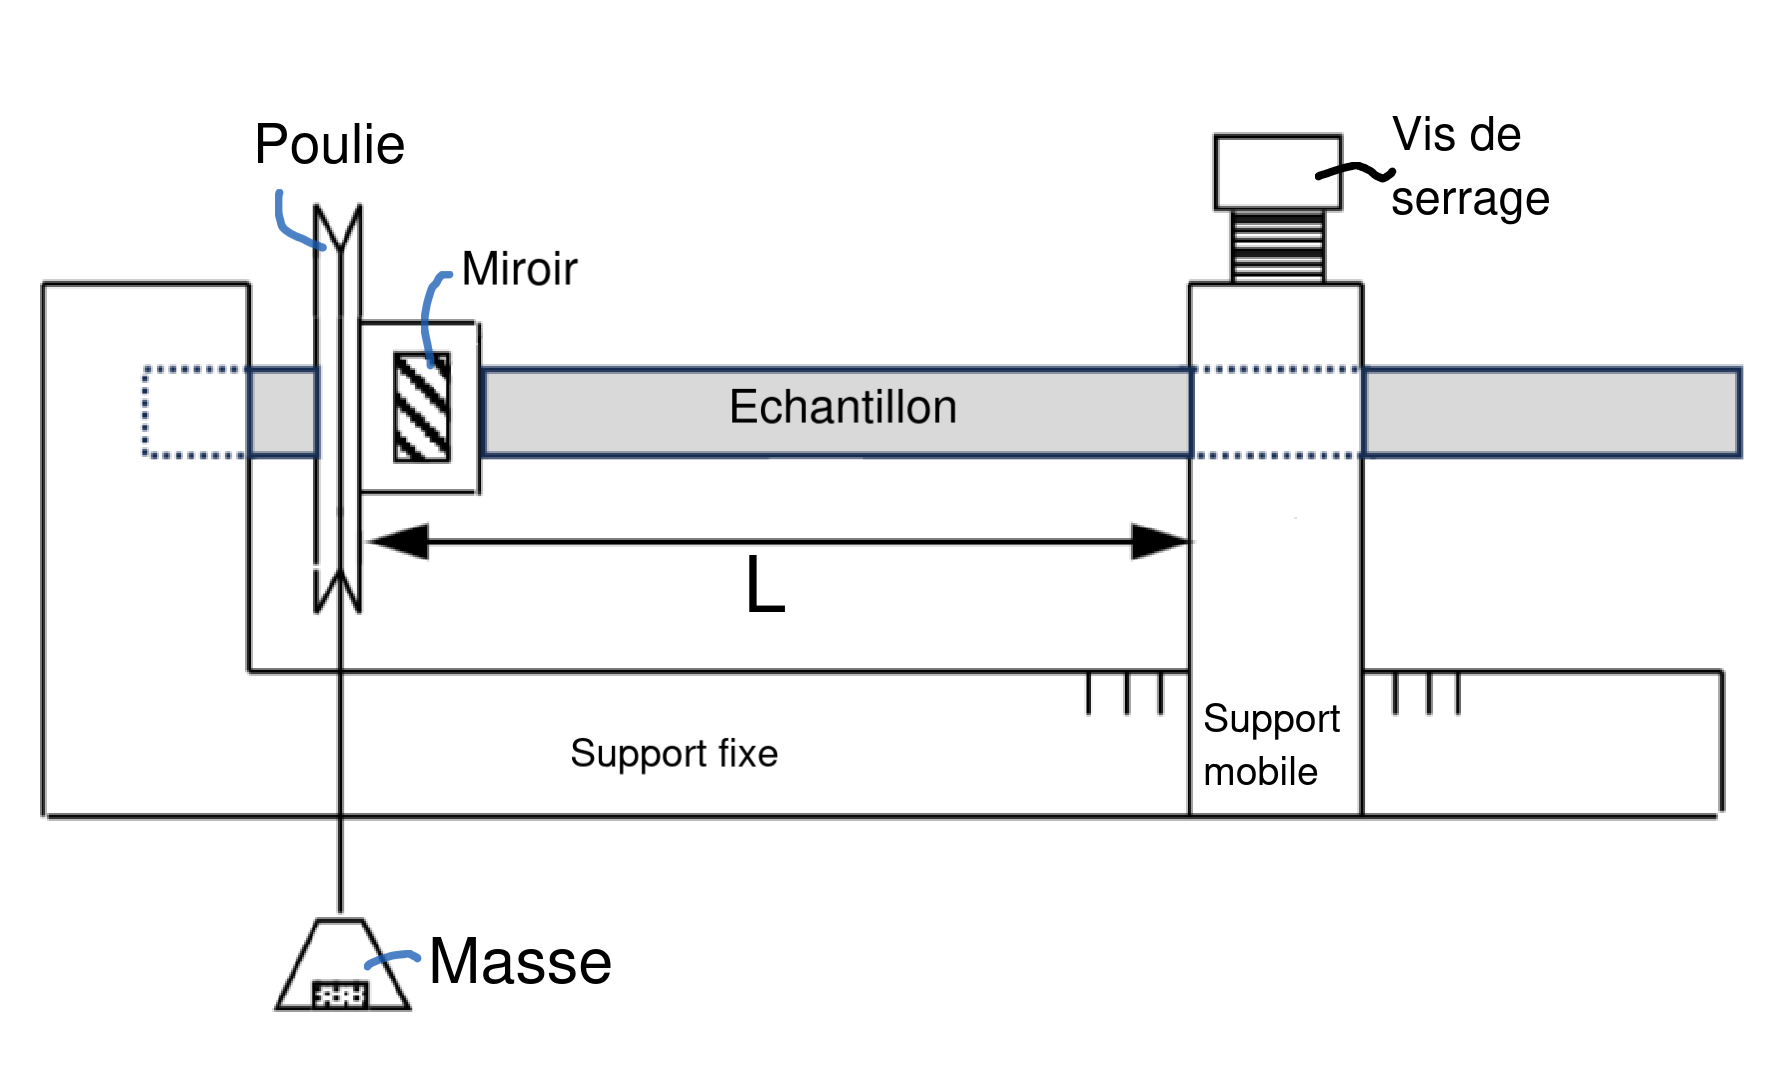
\includegraphics[width=0.6\linewidth]{figures/statique_annotated.png}
    \caption{Montage pour la méthode statique \cite{notice}}
    \label{fig:montage_statique}
\end{figure}

La méthode statique est appliquée à des échantillon cylindriques d'épaisseur $d$. Elle permet de mesurer le comportement de l'échantillon en changeant certains paramètres. Le montage est présenté à la \autoref{fig:montage_statique}. Un échantillon est placé en rotation libre du coté gauche et fixé du coté droit. Le miroir permet de refleter un laser sur une règle afin de déterminer l'angle de torsion de l'échantillon. Il est alors possible de faire varier 2 paramètres:
\begin{itemize}
    \item La longueur $L$ de l'échantillon
    \item Le poids $P=mg$ accroché à la poulie de diamètre $D$
\end{itemize}
L'angle de déformation est alors donné par
\begin{equation}
    \theta = \frac{1}{2}\arctan\left(\frac{\delta}{a}\right)
    \label{eq:angle_deformation}
\end{equation}
où $\delta$ est la déviation du laser et $a$ est la distance miroir-règle. Le facteur $1/2$ vient du fait  que le laser est dévié d'un angle $2\theta$.

Une régression linéaire sur les mesures longueur-angle ou poids-angle permet alors de déterminer le module de cisaillement à l'aide de l'\autoref{eq:module_cisaillement_statique}, en exprimant $\theta$ en fonction des paramètres qui ont été variés.

\subsection{Méthode dynamique}

\begin{wrapfigure}{R}{0.4\linewidth}
    % WARNING
    \vspace*{-2cm}
    \centering
    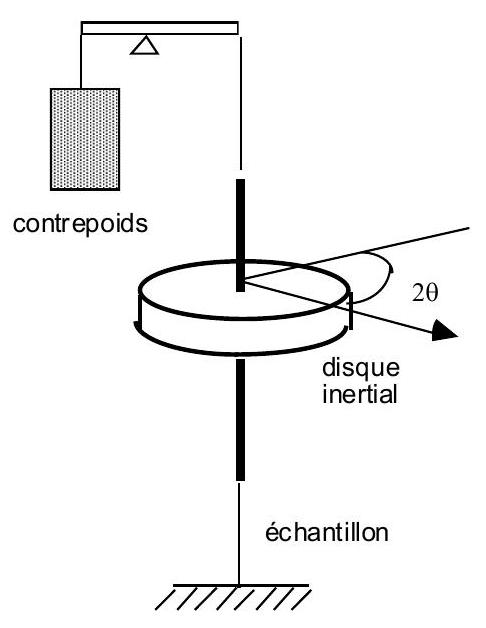
\includegraphics[width=\linewidth]{figures/dynamique.png}
    \caption{Montage pour la méthode dynamique \cite{notice}}
    \label{fig:montage_dynamique}
    \vspace*{-1.5cm}
\end{wrapfigure}
La méthode dynamique s'applique sur des échantillons en forme de fil, de longueur constante $\ell$ et épaisseur $d$. Le montage présenté à la \autoref{fig:montage_dynamique} constitue un pendule de torsion. L'échantillon est suspendu à l'extrémité d'un fil, auquel est attaché un disque de moment d'inertie $I$. Sachant que différents matériaux vont donner différentes pulsations, la mesure de la periode d'oscillation permet de déterminer le module de cisaillement de l'échantillon à l'aide de l'\autoref{eq:module_cisaillement_dynamique}. La période est mesurée avec un système de miroir et laser similaire au montage précédent.

De plus, la décroissance de l'amplitude des oscillation en fonction du temps permet de déterminer le coefficient d'amortissement $\lambda$ du matériau, en utilisant l'\autoref{eq:decrement_log}.

